\subsection{tempPerDay()}

The third graph we created was the second example graph proposed in the instructions file. It shows the mean temperature for each day of the year. It is produced by the member function of tempTrender called "tempPerDay(). It is akin to stacking 365 of the "tempOnDay()" histograms vertically. 

\begin{figure}[h]
\centering
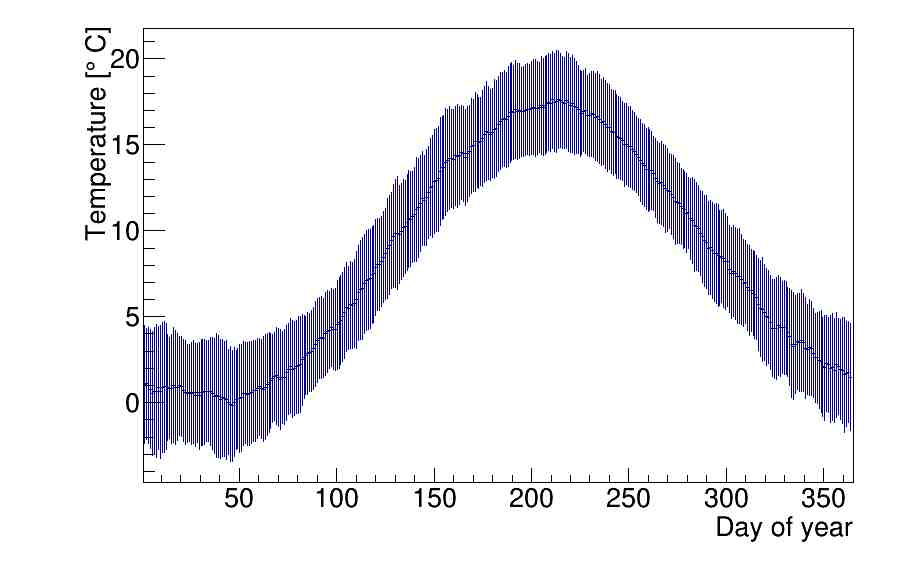
\includegraphics[scale=0.3]{graph3.png}
\caption{Histogram showing the mean temperature on each day of the year. Produced by "tempPerDay()". }
\end{figure}